\chapter{Prototyping}
%Introduction
This prototype exemplifies the use of Java RMI Clients and Servers. As well as showing the basics of Remote Method Invocation, a basic leader-election algorithm is implemented. This leader-election takes place if it is discovered, that the current leader has gone down.

In the prototype the leader, and only the leader, will register the function "GloriousLeader" on the RMI Registry. 
If the leader goes down, a new leader will be elected this will ReBind its own GloriousLeader function.

In perspective, the GloriousLeader function should access something that required a single-node access. In this basic prototype, the function returns the NodeID of the leader node as well as short message (as a String object).

\section{System setup}
\subsection{Setting up RMI Registry}
The host machine must host the RMI registry, the service in charge of serving up Remote Method calls.
The RMI Registry uses the CLASSPATH variable to identify the Java classes/methods bound and requested from the host. 

Therefore, the CLASSPATH variable must be set:

\begin{center}
	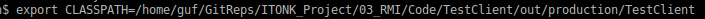
\includegraphics[width=\textwidth]{ExportingClasspath.png}
	\captionof{figure}{Exporting the CLASSPATH variable on Linux}
\end{center}

This is the path to the base directory of the .class files, compiled with the Java Compiler (Through IntelliJ).

The RMI registry is created programatically from within the SystemInitializerMain class' main function, which is responsible for initializing the system. 

The RMI registry needs to know the network interface it will communicate on. This is done through setting the system property \textit{java.rmi.server.hostname} to the external IP of the host machine. 

\begin{center}
	\fbox{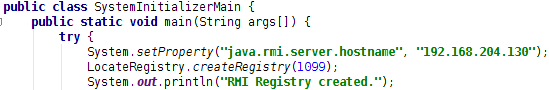
\includegraphics[scale=1]{SetPropertyMain.png}}
	\captionof{figure}{Creating the RMI registry and setting the appropriate properties java.rmi.server.hostname}
\end{center}

\subsection{Running the Servers}
When starting the main programs, java needs to know the path to the .class files of the project. The java.rmi.server also needs to know the path to the actual .class files.

This is done by specifying the java.rmi.server.codebase property. This is done using the java -D[Property]=[Value] parameter.

\section{System description}
The system consists of nodes in a ring-like configuration.

Each node can be either a leader or a slave Node. 
\subsection{Node}
The node is the main entity in the system. Each node has the capacity for being both leader and slave. 

All nodes has a Server and a Client object. After a leader election, if a Node declares itself the leader, it will create a LeaderClass object for itself. 

The Node class exposes methods for interacting with the Server and Client objects.

\begin{center}
	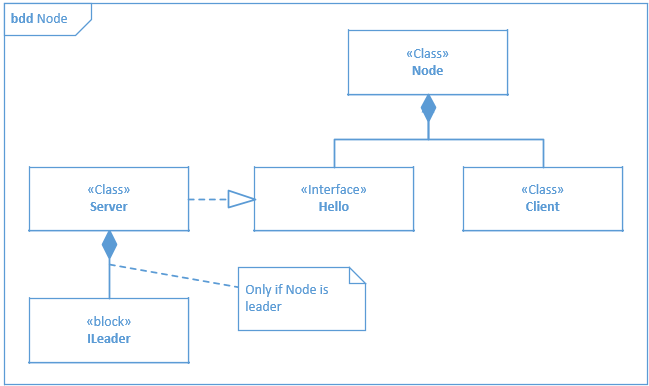
\includegraphics[scale=1]{NodeBDD.png}
	\captionof{figure}{Block Definition Diagram of the Node class}
\end{center}

When a Node comes online, it will trigger a leader election. This is done to make sure that even if new nodes come online, the one with the highest id will be the leader.

\subsubsection{Hello Interface}
This interface is implemented by the Server class. The interface exposes functions for leader elections as well as organization messages needed for setting the current leader etc.

This is used for creating the stub, used by other servers for calling other serves when doing leader election.

\begin{center}
	\fbox{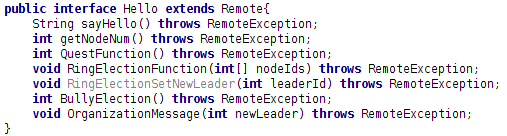
\includegraphics[scale=1]{HelloInterface.png}}
	\captionof{figure}{Definition of the Hello interface}
\end{center}

\subsubsection{Server}
The Server object takes care binding and serving up functions. The Server implements the Hello interface. See BDD of the Node class.

When the Server comes online it registers itself to the RMI registry with id "QuestNodeXX" where XX is the ID of the node, that owns the Server. This is done in the servers constructor:

\begin{center}
	\fbox{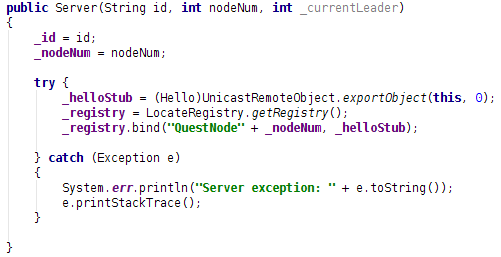
\includegraphics[width=\textwidth]{ServerConstructor.png}}
	\captionof{figure}{Constructor for the Server class}
\end{center}


The main purpose of the Server is to expose:

\begin{itemize}
\item Questing Methods for leader elections
\item OrganizationMessage(\textit{int leaderID})
\end{itemize}

If the node is Leader, the Server owns a LeaderClass object that exposes the GloriousLeader function. 

\subsubsection{Client}
The Client class is the entity in charge of calling the GloriousLeader function, after looking up the RMI registry.

The CallGloriousLeader() makes a lookup in the RMI registry, to find the leader function. It calls the function and prints the response.

\begin{center}
	\fbox{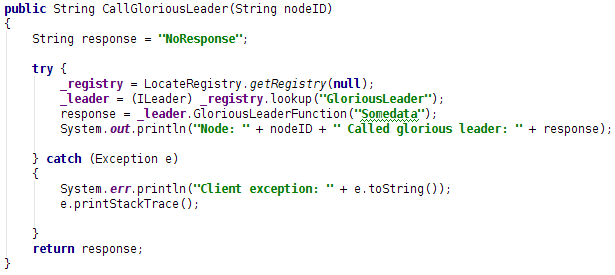
\includegraphics[width=\textwidth]{ClientCallGloriousLeader.png}}
	\captionof{figure}{CallGloriousLeader in the Client class}
\end{center}

If the leader cannot be reached, the Client will tell the node to start an election. 

\subsubsection{ILeader}
The ILeader interface is the interface for the Leader and exposes the GloriousLeader function. This interface is used to create the RMI stub of the LeaderClass in the Client objects.

\begin{center}
	\fbox{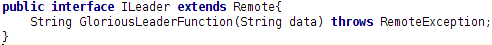
\includegraphics[width=\textwidth]{ILeaderInterface.PNG}}
	\captionof{figure}{The ILeader interface definition}
\end{center}

The GloriousLeader function throws the RemoteException if something goes wrong. This is strictly necessary to detect when something goes wrong in the transmission and a leader election is necessary.

\subsubsection{LeaderClass}
This is the implementation of the ILeader interface. This class is created when a Node is elected leader.

Upon creation, the LeaderClass checks, if the "GloriousLeader" id is found in the RMI registry. If it is found it will be unbound by the Registry.UnBind(String) function. 

The LeaderClass will then rebind itself as the "GloriousLeader", so that the current Node is now in charge of the GloriousLeader function.

\begin{center}
	\fbox{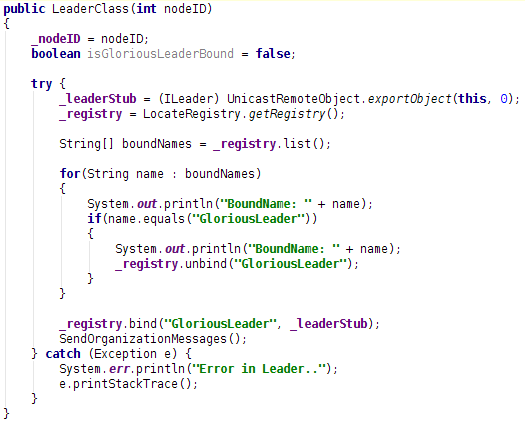
\includegraphics[scale=1]{LeaderClassConstructor.png}}
	\captionof{figure}{The LeaderClass Constructor}
\end{center}

When the new leader is bound, it will send out organization messages with the new leader ID, using the SendOrganizationMessages function.

\section{Leader Election}
In the prototype, the leader is in charge of exposing the GloriousLeader method to the other nodes in the system. In a real system, this function could be in charge of distributing workloads, accessing a database etc. In this prototype the leader's GloriousLeader function just returns the ID of the node it belongs to along with a small message. 

\subsection{GloriousLeader function}
The GloriousLeader function is very simply implemented:

\begin{center}
	\fbox{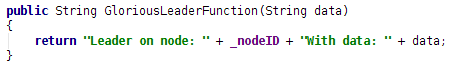
\includegraphics[scale=1]{GloriousLeaderFunction.png}}
	\captionof{figure}{The GloriousLeaderFunction implementation}
\end{center}


\subsection{Bully implementation}
The Bully Election implementation is actually quite straight forward. It is implemented as a single function as described below.

\subsubsection{StartBullyElection function}
When a node discovers that the leader has terminated it will execute this function. It basically just calls this function on all nodes with a higher ID number. If no one replies and "responseID" therefore is -1 then that node is elected as the new leader and runs the SetLeader() function to tell the others who the new leader is. 

\begin{center}
	\fbox{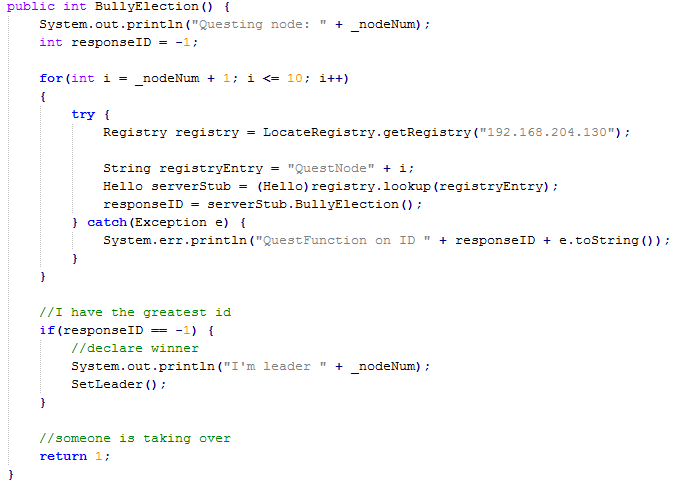
\includegraphics[width=\textwidth]{StartBullyElection.PNG}}
	\captionof{figure}{The StartBullyElection implementation}
\end{center}

\subsection{Ring implementation}
The ring election is implemented with three functions. It must be possible to trigger a new election when a node fails to respond. During this process each node mush be able to handle two kinds of messages. The first is the election process, where a node receives a message containing the ID's from all previously nodes in the ring. The node appends its own id to the message and passes it along the ring:

\begin{center}
	\fbox{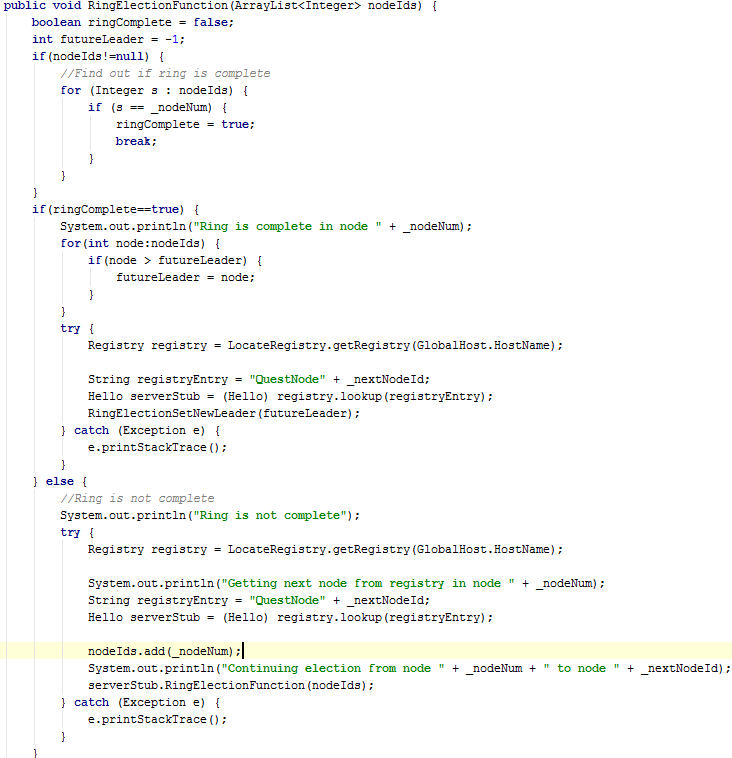
\includegraphics[width=\textwidth]{RingElection_Function.PNG}}
	\captionof{figure}{The RingElectionFunction implementation}
\end{center}

If the id is already in the message, the ring must be completed. If this is the case the node elects a new leader and starts the notification process about the new leader.

This is done using the RingElectionSetNewLeader function. The node is notified about who is the new leader, saves this information and parses it on. When the message returns to the node that started the message, the ring is complete.

\begin{center}
	\fbox{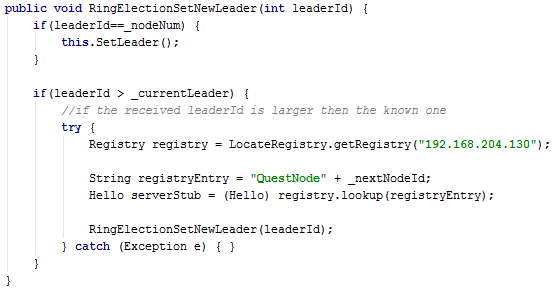
\includegraphics[width=\textwidth]{RingElection_SetNewLeader.PNG}}
	\captionof{figure}{The SetNewLeader implementation of ring election}
\end{center}



\subsubsection{[QUESTING FUNCTION]}
\subsection{Optimized Bully}
\subsubsection{QuestingFunction}




\begin{center}
	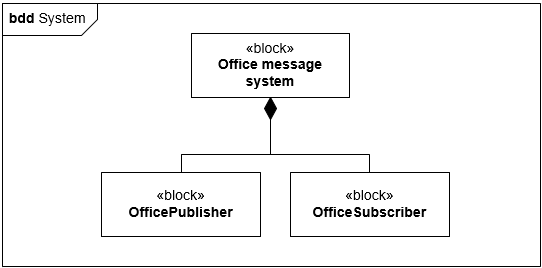
\includegraphics[width=\textwidth]{bdd_image.png}
	\captionof{figure}{BDD of the Office Message System}
\end{center}
\section{Tests}
\subsection{Starting InitializerMain}
The InitializerMain class creates the RMI registry with the correct properties. The main function in this class must be run before anything else. 

\begin{center}
	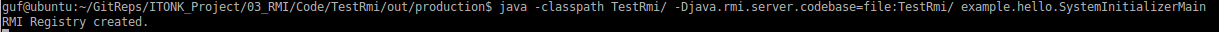
\includegraphics[width=\textwidth]{StartingSystemInitializerMain.png}
	\captionof{figure}{Starting the SystemInitializerMain through Linux console}
\end{center}

In the definition of this project, it was to be assumed that each node knows the number of nodes that \textit{should} be present in the system (here assumed to be 11).

\subsection{The Main function}
The main function for starting nodes takes the node id as an argument. This way the node id can be passed to the node on startup of the process. Also this way, each node runs in its own process.

\begin{center}
	\fbox{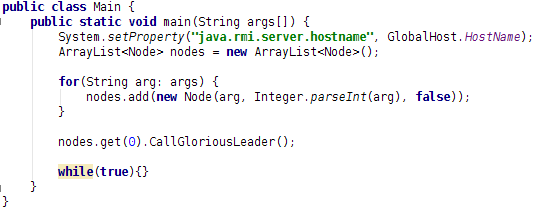
\includegraphics[width=\textwidth]{MainNodeStarter.png}}
	\captionof{figure}{Implementation of the main function of the Main class}
\end{center}

Note that the Node calls GloriousLeader when it comes online. 

\subsection{Ring Election Test}

\subsection{Bully Election Test}
For this test, the InitializerMain has been started. Initially no nodes, and therefore no leader, is present. 

The first Node started has id 1.

\begin{center}
	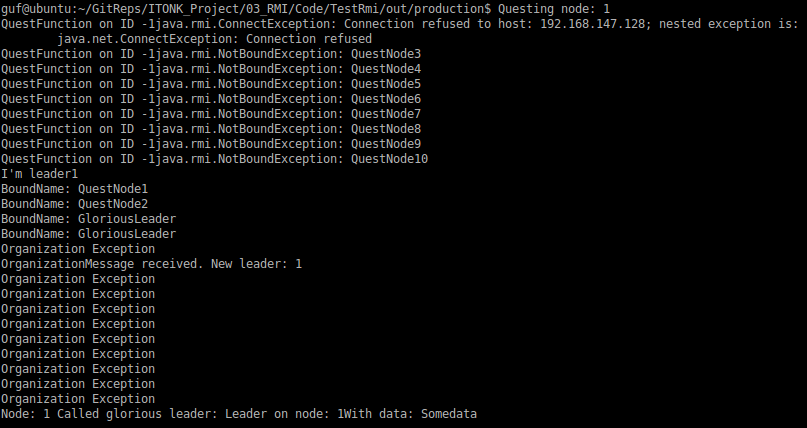
\includegraphics[width=\textwidth]{StartingNode1Bully.png}
	\captionof{figure}{Starting Node 1}
\end{center}

All election messages are \textbf{not} printed to the console, as this would be impossible to show all these messages in a report.

It can be seen, that the node elects itself as leader (as it cannot get contact to any other nodes) and then calls the GloriousLeader function on itself. 

The next Node started has id 8 and should therefore be elected leader.

\begin{center}
	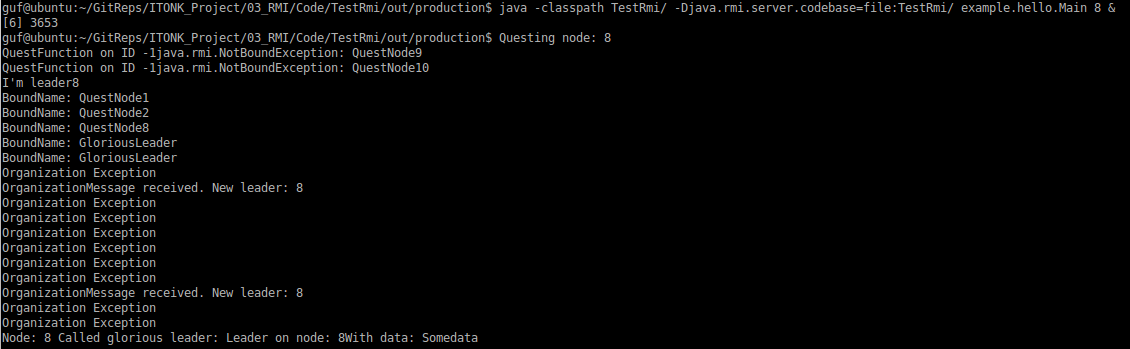
\includegraphics[width=\textwidth]{StartingNode8Bully.png}
	\captionof{figure}{Starting Node 1}
\end{center}

Node 8 is elected leader. 

When adding a node with a lower id (here 6):

\begin{center}
	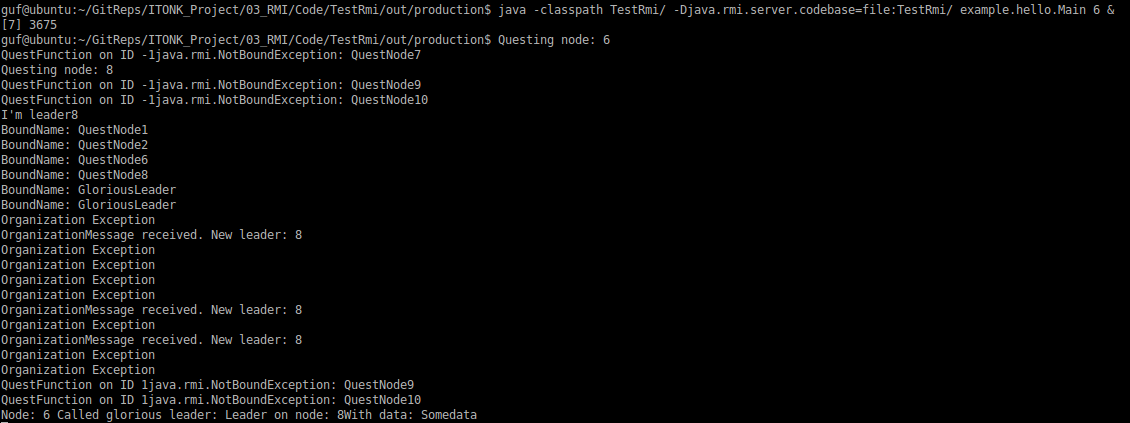
\includegraphics[width=\textwidth]{StartingNode6Bully.png}
	\captionof{figure}{Starting Node 1}
\end{center}

Node 8 is still elected leader, as it had a higher ID than 6.

When a node attempts to call GloriousLeader function, when the leader process has been killed, this should trigger a leader election. 

[INSERT IMAGE OF LEADER ELECTION BEING TRIGGERED BY ERROR]

\subsection{Optimized Bully Test}
